\chapter{Current of Electricity}

\section{Electric Current}

\begin{definition}
    \vocab{Electric current} ($I$) is the rate of flow of charge. \[I = \der{Q}{t}.\]
\end{definition}

The SI unit of electric current is the ampere (A).

\begin{definition}
    An \vocab{electric conductor} is a material that contains mobile charge carriers (e.g. electrons). Else, it is an \vocab{electric insulator}.
\end{definition}

Electric current is conventionally taken to be in the direction of the flow of positively-charged particles, even though in many conductors, negatively charged electrons or ions are the charge carriers.

\begin{proposition}
    The current $I$ in a wire is given by \[I = nAvq,\] where $n$ is the number of charge carriers per volume, $A$ is the cross-sectional area of the wire, $v$ is the drift velocity of the charge carriers, and $q$ is the charge on each charge carrier.
\end{proposition}
\begin{proof}
    Let $V$ be the volume of the wire and $l$ the length of the wire, so $V = Al$. Let $N$ be the total number of charge carriers. Then the total charge $Q$ is given by \[Q = \text{charge per charge carrier} \times \text{total number of charge carriers} = \bp{q}\bp{nV} = qnAl.\]

    Assuming constant charge, we have from the definition of $I$ that \[I = \frac{Q}{t} = \frac{qnAl}{t} = qnA \bp{\frac{l}{t}} = qnAv.\]
\end{proof}

\section{Potential Difference and Electromotive Force}

\begin{definition}
    The \vocab{potential difference} ($V$, p.d.) or \vocab{voltage} between two points in a circuit is the work done per unit charge when electrical energy is transferred to non-electrical energy when the charge passes from one point to the other. \[V = \frac{W}{Q}.\]
\end{definition}

The SI unit of potential difference is the volt (V).

\begin{definition}
    The electromotive force ($E$, e.m.f.) of a source is the work done per unit charge when non-electrical energy is transferred into electrical energy when the charge is moved round a complete circuit.
\end{definition}

The SI unit of electromotive force is the volt (V).

Note that the electromotive force is a source of energy and will always exist, even when a current is not flowing in the circuit. However, potential difference exists only when current is flowing in the circuit.

\section{Resistance}

\begin{definition}
    The \vocab{resistance} ($R$) of a conductor is the ratio of the potential difference across the conductor to the current passing through it. \[R = \frac{V}{I}.\]
\end{definition}

The SI unit of resistance is the ohm ($\O$).

\begin{law}[Ohm's Law]
    A current $I$ flowing through a conductor is directly proportional to the potential difference $V$ applied across the conductor, provided that physical conditions (like temperature, stress of the material, etc.) remain constant. \[I \propto V.\]
\end{law}

\begin{definition}
    The \vocab{resistivity} ($\rho$) of a material is a measure of its resistance to current flowing through it. It relates the resistance $R$ of the material to its length $l$ and cross-sectional area $A$ via \[R = \rho \frac{l}{A}.\]
\end{definition}

The SI unit of resistivity is ohm metre ($\O$ m).

\subsection{$I$-$V$ Characteristics}

The $I$-$V$ characteristic (or $I$-$V$ curve) shows how the current $I$ flowing through a device varies with the voltage $V$ across it.

When the current passing through a material increases, the temperature of the material is likely to increase. Two main changes occur at the molecular level which affects the resistance of the material:
\begin{itemize}
    \item the number of charge carriers per unit volume ($n$) increases, which reduces the resistance of the material.
    \item the thermal vibrations of the lattice atoms increases, which increases the number of collisions between the charged carriers and the lattice atoms. This reduces the drift velocity $v$ of the charged carriers, hence increasing the resistance of the material.
\end{itemize}

Depending on the nature of the material, one effect may dominate, which will determine the variation of $I$ with respect to $V$.

\subsubsection{Ohmic Resistors}

An \vocab{ohmic resistor} refers to a resistor with a constant resistance.

Note that ohmic resistors obey Ohm's law, where $1/R$ is the constant of proportionality between $I$ and $V$: \[I = \frac{V}{R}.\]

The $I$-$V$ characteristic of an ohmic resistor is a straight line through the origin.

\begin{figure}[H]
    \centering
    \begin{tikzpicture}[scale=0.7, trim axis left, trim axis right]
        \begin{axis}[
            domain=0:3,
            axis equal image,
            axis y line=middle,
            axis x line=middle,
            xtick = \empty,
            ytick = \empty,
            xlabel = {$V$},
            ylabel = {$I$},
            legend cell align={left},
            legend pos=outer north east,
            ]

            \addplot [samples=200,red, very thick] {x};
        \end{axis}
    \end{tikzpicture}
    \caption{The $I$-$V$ characteristic of an ohmic resistor.}
\end{figure}

A metallic conductor at constant temperature is an example of an ohmic resistor. At constant temperature, its lattice vibrations remain the same, and so its resistance remains the same.

\subsubsection{Filament Lamp}

The $I$-$V$ characteristic of a filament lamp is increasing but concave downwards.

\begin{figure}[H]
    \centering
    \begin{tikzpicture}[scale=0.7, trim axis left, trim axis right]
        \begin{axis}[
            domain=0:2,
            axis equal image,
            axis y line=middle,
            axis x line=middle,
            xtick = \empty,
            ytick = \empty,
            xlabel = {$V$},
            ylabel = {$I$},
            legend cell align={left},
            legend pos=outer north east,
            ]

            \addplot [samples=200,red, very thick] {ln(1+x)};
            \addplot[samples=200, dashed] {x};
        \end{axis}
    \end{tikzpicture}
    \caption{The $I$-$V$ characteristic of a filament lamp.}
\end{figure}

As temperature increases, the number of electrons in a filament lamp does not vary significantly. However, lattice vibrations increases, which reduces the drift velocity of electrons, hence leading to an increase in resistance.

\subsubsection{Semiconductor Diode}

A \vocab{diode} is a device that has a low resistance in one direction and a very high resistance in the other direction.

If a potential difference is applied across a diode in the direction with low resistance, it is said to be \vocab{forward biased}. If a potential difference is applied in the direction with very high resistance, it is said to be \vocab{reverse biased}.

The $I$-$V$ characteristic of a semiconductor diode is increasing and concave upwards when forward biased. When reverse biased, the $I$-$V$ cure is almost zero, except when the voltage exceeds the breakdown voltage and the current becomes very large.

\begin{figure}[H]
    \centering
    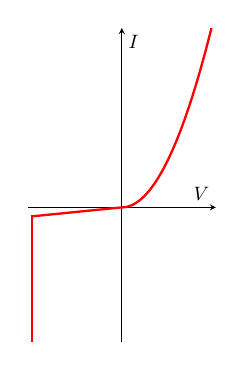
\begin{tikzpicture}[scale=0.7, trim axis left, trim axis right]
        \begin{axis}[
            xmin=-2.1,
            xmax=2.1,
            ymax=4,
            ymin=-3,
            axis equal image,
            axis y line=middle,
            axis x line=middle,
            xtick = \empty,
            ytick = \empty,
            xlabel = {$V$},
            ylabel = {$I$},
            legend cell align={left},
            legend pos=outer north east,
            ]

            \addplot [samples=200,red, very thick, domain=0:2] {x^2};
            \addplot [samples=200,red, very thick, domain=-2:0] {0.1*x};
            \draw[red, very thick] (-2, -0.18) -- (-2, -3);
        \end{axis}
    \end{tikzpicture}
    \caption{The $I$-$V$ characteristic of a semiconductor diode.}
\end{figure}

Consider the forward biased region of the $I$-$V$ graph. As $V$ increases, the temperature of the semiconductor increases, hence electrons have more energy and are more likely to escape from atoms. This increases $n$ significantly. At the same time, there is also an increase in the rate of interaction of electrons with the lattice vibrations. However, the increase in $n$ predominates over the rate of lattice interactions, hence the overall effect is that resistance decreases.

\subsubsection{Negative Temperature Coefficient Thermistor}

A \vocab{thermistor} is a resistor with a resistance that is temperature dependent. A negative temperature coefficient (NTC) thermistor is a thermistor whose resistance decreases with temperature.

The $I$-$V$ characteristic of an NTC thermistor is increasing and concave upwards.

\begin{figure}[H]
    \centering
    \begin{tikzpicture}[scale=0.7, trim axis left, trim axis right]
        \begin{axis}[
            domain=0:2,
            axis equal image,
            axis y line=middle,
            axis x line=middle,
            xtick = \empty,
            ytick = \empty,
            xlabel = {$V$},
            ylabel = {$I$},
            legend cell align={left},
            legend pos=outer north east,
            ]

            \addplot [samples=200,red, very thick] {0.5*x^2};
        \end{axis}
    \end{tikzpicture}
    \caption{The $I$-$V$ characteristic of a NTC thermistor.}
\end{figure}

As $V$ increases, the temperature of the NTC thermistor increases, resulting in lower resistance.

\section{Power}

\begin{proposition}
    The power $P$ dissipated between two points is given by the product of the potential difference $V$ and the current $I$ between the two points, i.e. $P = IV$.
\end{proposition}
\begin{proof}
    From the definition of potential difference, \[V = \frac{W}{Q} = \frac{W/t}{Q/t} = \frac{P}{I},\] which rearranges to $P = IV$.
\end{proof}

\begin{corollary}
    The power $P$ is given by \[P = I^2 R = \frac{V^2}{R}.\]
\end{corollary}
\begin{proof}
    Recall that $V = IR$, so \[P = IV = I\bp{IR} = I^2 R \quad \tand \quad P = IV = \bp{\frac{V}{R}}V = \frac{V^2}{R}.\]
\end{proof}

\section{Internal Resistance}

In practice, whenever there is a current, some of the energy transferred by a source is dissipated in the source itself. The source is said to have \vocab{internal resistance} ($r$).

The internal resistance of a source could be depicted in a circuit diagram as a resistor $r$ connected in series with an ideal source of electromotive force $E$, connected to an external circuit of combined resistance $R$.

\begin{figure}[H]
    \centering
    \includegraphics[scale=0.4]{media/Internal Resistance.jpg}
    \caption{A simplified circuit diagram showing the internal resistance of a source.\protect\footnotemark}
\end{figure}
\footnotetext{Source: \url{https://thescienceandmathszone.com/internal-resistance/}}

As the electromotive force is the total energy (per unit charge) available to the circuit and some energy is dissipated due to internal resistance, the potential difference available to the external circuit will be less than the electromotive force.

\begin{proposition}
    The potential difference $V$ available to the external circuit is given by \[V = E - Ir.\]
\end{proposition}
\begin{proof}
    Conservation of energy implies that the electromotive force $E$ must be equal to the sum of the potential difference across the external and internal resistances, i.e. \[E = IR + Ir = V + Ir \implies V = E - Ir.\]
\end{proof}

Various quantities can be expressed in terms of $E$, $r$ and $R$.

\begin{proposition}
    \phantom{.}
    \begin{itemize}
        \item Current $\displaystyle I = \frac{E}{R + r}$
        \item Terminal potential difference $\displaystyle V = IR = \frac{RE}{R+r}$.
        \item Total power dissipated in the complete circuit $\displaystyle P_T = IE = \frac{E^2}{R+r}$.
        \item Power dissipated in the external circuit $\displaystyle P_R = IV = \frac{R E^2}{(R+r)^2}$.
        \item Efficiency $\displaystyle \eta = \frac{P_R}{P_T} = \frac{R}{R+r}$.
    \end{itemize}
\end{proposition}

\begin{theorem}[Maximum Power Transfer Theorem]
    Maximum power is supplied to the external circuit when the resistance of the external circuit is equal to the internal resistance of the source.
\end{theorem}
\begin{proof}
    From above, we see that the power dissipated in the external circuit is \[P_R = \frac{R E^2}{(R+r)^2}.\] By the AM-GM inequality, \[(R+r)^2 \geq 4Rr \implies P_R = \frac{RE^2}{(R+r)^2} \leq \frac{RE^2}{4Rr} = \frac{E^2}{4r},\] which depends only on the source. Equality occurs when $R = r$, as desired.
\end{proof}